%! Author = drakanoy
%! Date = 10.09.2024

% Preamble
\documentclass[12pt]{article}

% Packages
\usepackage[utf8]{inputenc}
\usepackage[T2A]{fontenc}
\usepackage[english, russian]{babel}
\usepackage[a4paper, includefoot, left=1.5cm, right=1.5cm, top=1cm, bottom=1.5cm, headsep=1cm, footskip=1cm]{geometry}
\usepackage{makecell}
\usepackage{amsmath}
\usepackage{graphicx}
\usepackage{enumitem}
\usepackage{svg}
\usepackage{multirow}
\usepackage{hyperref}
\usepackage{mathtools}
\usepackage{amssymb}
\usepackage{textcomp}
\usepackage{stmaryrd}

% Document
\begin{document}
\begin{large}
\begin{center}
\LARGE \textbf{Физика Конденсированного состояния}
\par
\LARGE \textbf{Кононов Александр Михайлович}
\par
    \textbf{1.03.2025}
\end{center}
\par \textbf{Задача 1}:
\par Условие:
\par
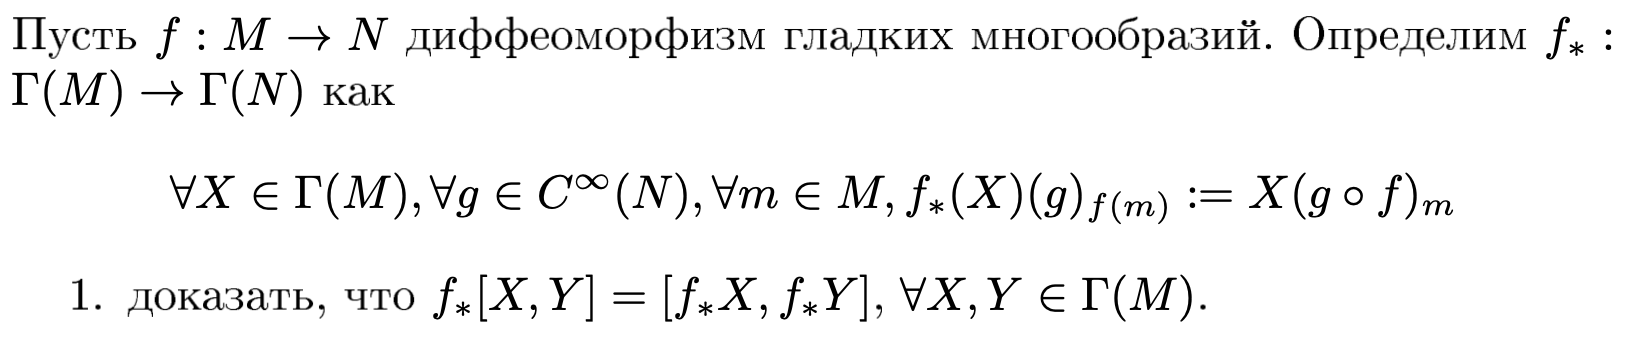
\includegraphics[width=1\textwidth]{photo_1.png}
%\begin{center}
%\underline{Рисунок 1}:
%\end{center}
\par Решение:
\par
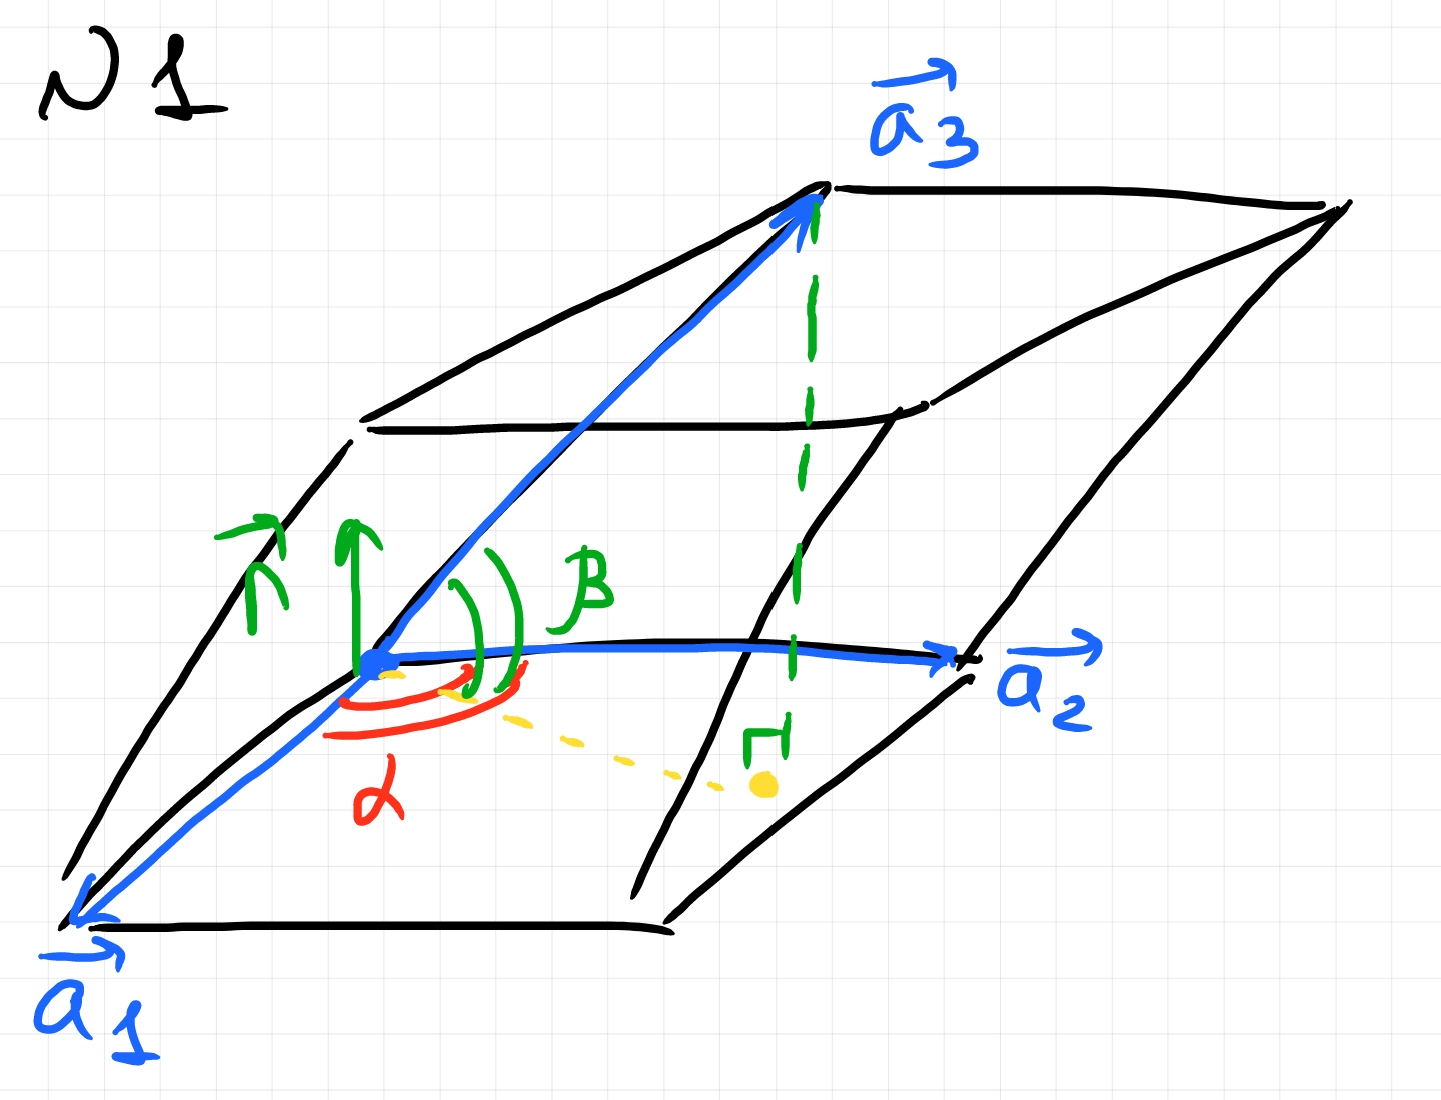
\includegraphics[width=1\textwidth]{photo_11.jpg}
\par
\par так как вектора образуют паралелепипед, его объем это
\[
    v_0 = S \cdot h
\]
из геометрии знаем
\[
    | \vec{a_1} \times \vec{a_2} | = |\vec{a_1}| \cdot |\vec{a_2}| \sin \alpha = S
\]
\[
    \vec{a_1} \times \vec{a_2} = \vec{n} \cdot S, \,\,\, \text{где} |\vec{n}| = 1
\]
\[
    \vec{a_3} \cdot \vec{n} = | \vec{n} | \cdot | \vec{a_3} | \cdot \cos(\pi/2 - \beta) = |\vec{a_3}|\sin \beta = h
\]
\[
    \Rightarrow (\vec{a_3} \cdot \left[ \vec{a_1} \times \vec{a_2} \right]) = S h = v_0
\]
QED
%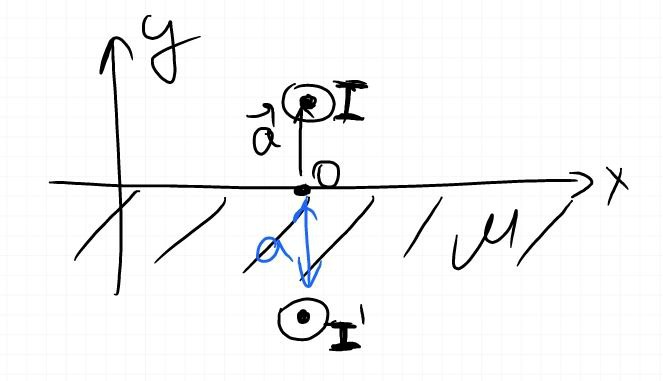
\includegraphics[width=1\textwidth]{photo_1.jpg}
%\par
%\begin{center}
%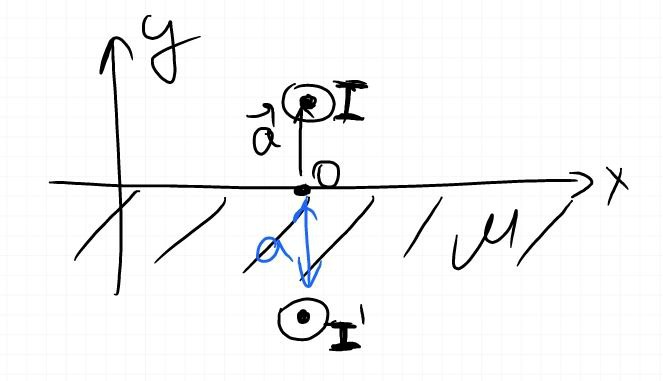
\includegraphics[width=0.4\textwidth]{photo_1.jpg}
%\end{center}

\par \textbf{Задача 2}:
\par Условие:
\par
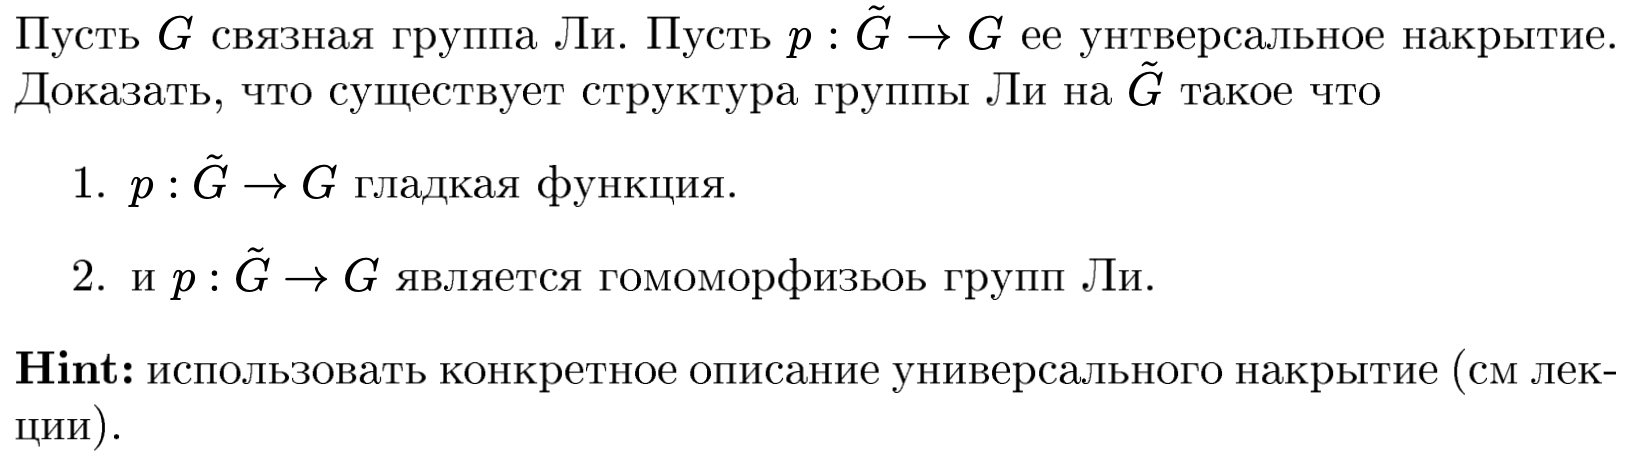
\includegraphics[width=1\textwidth]{photo_2.png}
\par Решение:
\par
\par В элементарной ячейке графена 2 атома (на картине элем ячейка обозначена красным)
\par
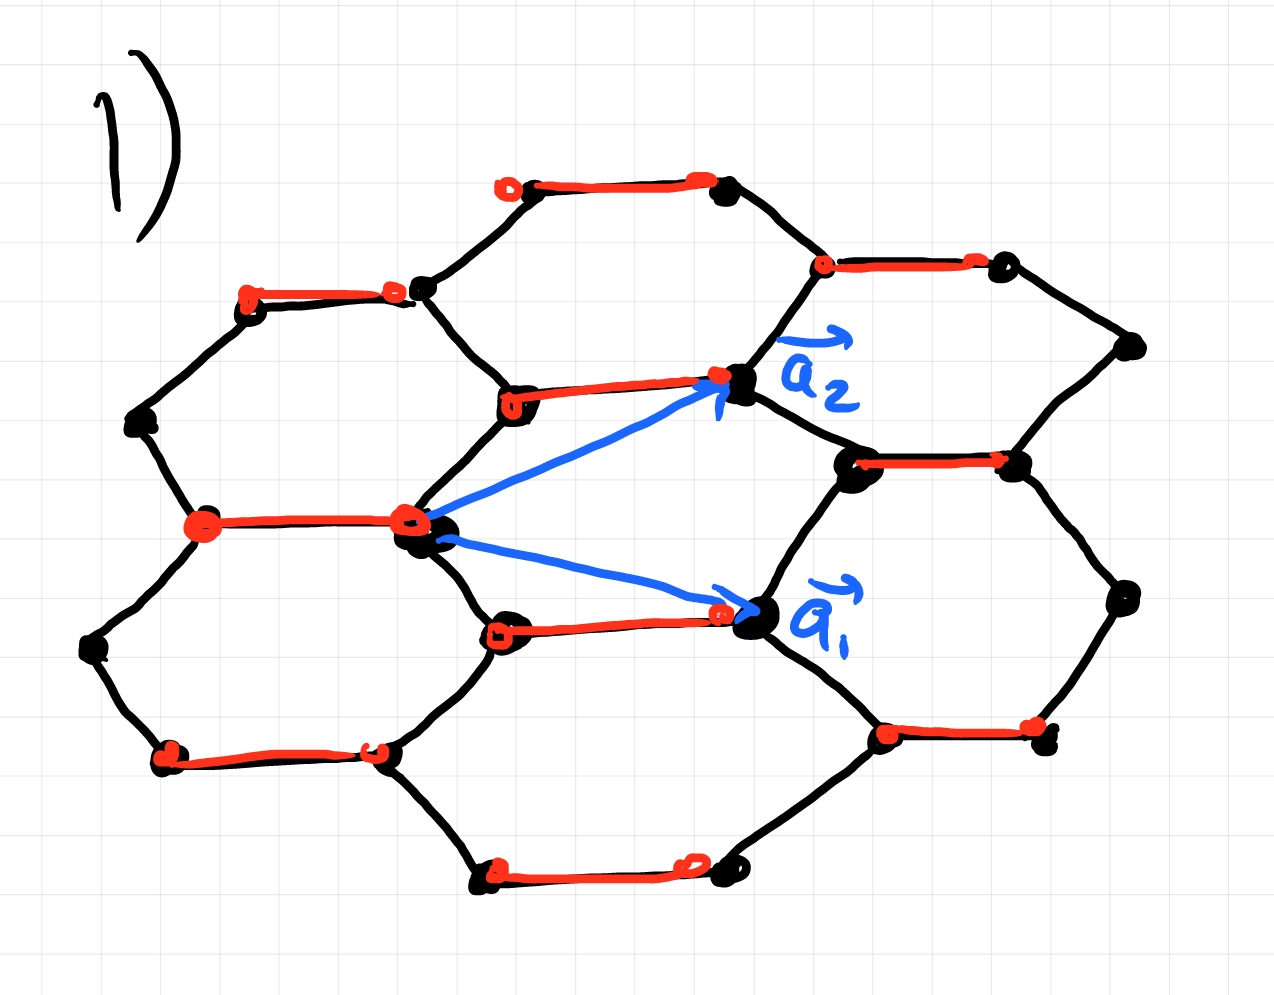
\includegraphics[width=0.7\textwidth]{photo_21.jpg}
\par
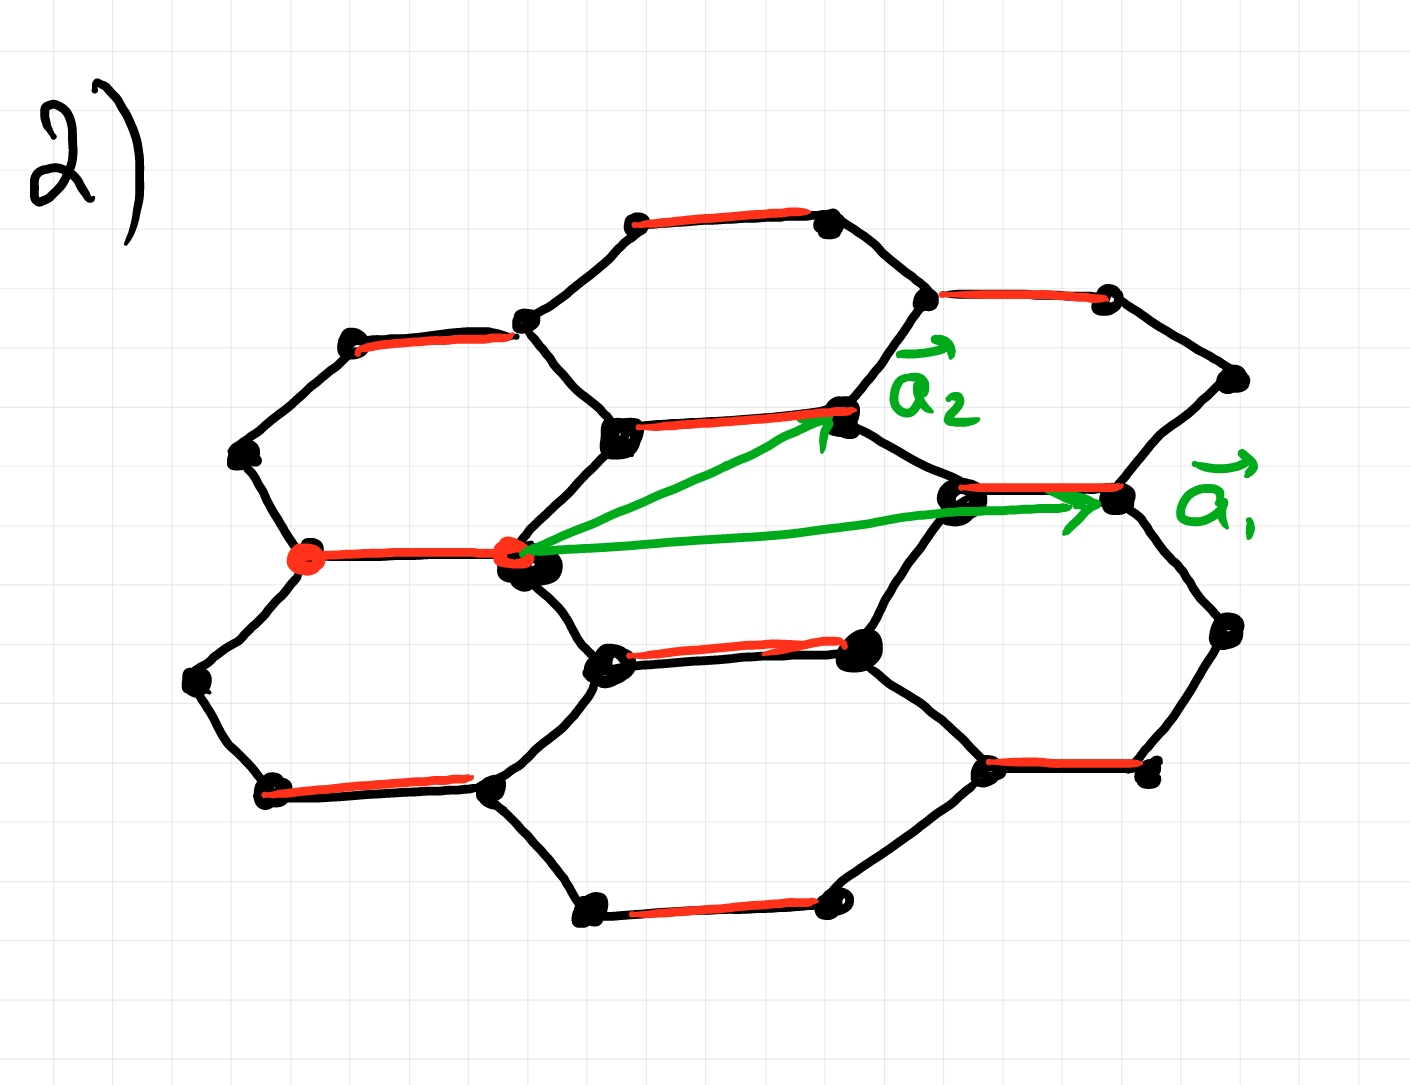
\includegraphics[width=0.7\textwidth]{photo_22.jpg}


\par \textbf{Задача 3}:
\par Условие:
\par
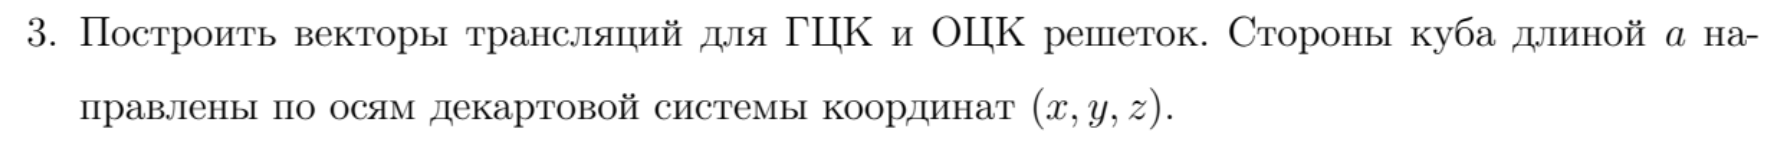
\includegraphics[width=1\textwidth]{photo_3.png}
\par Решение:
\par
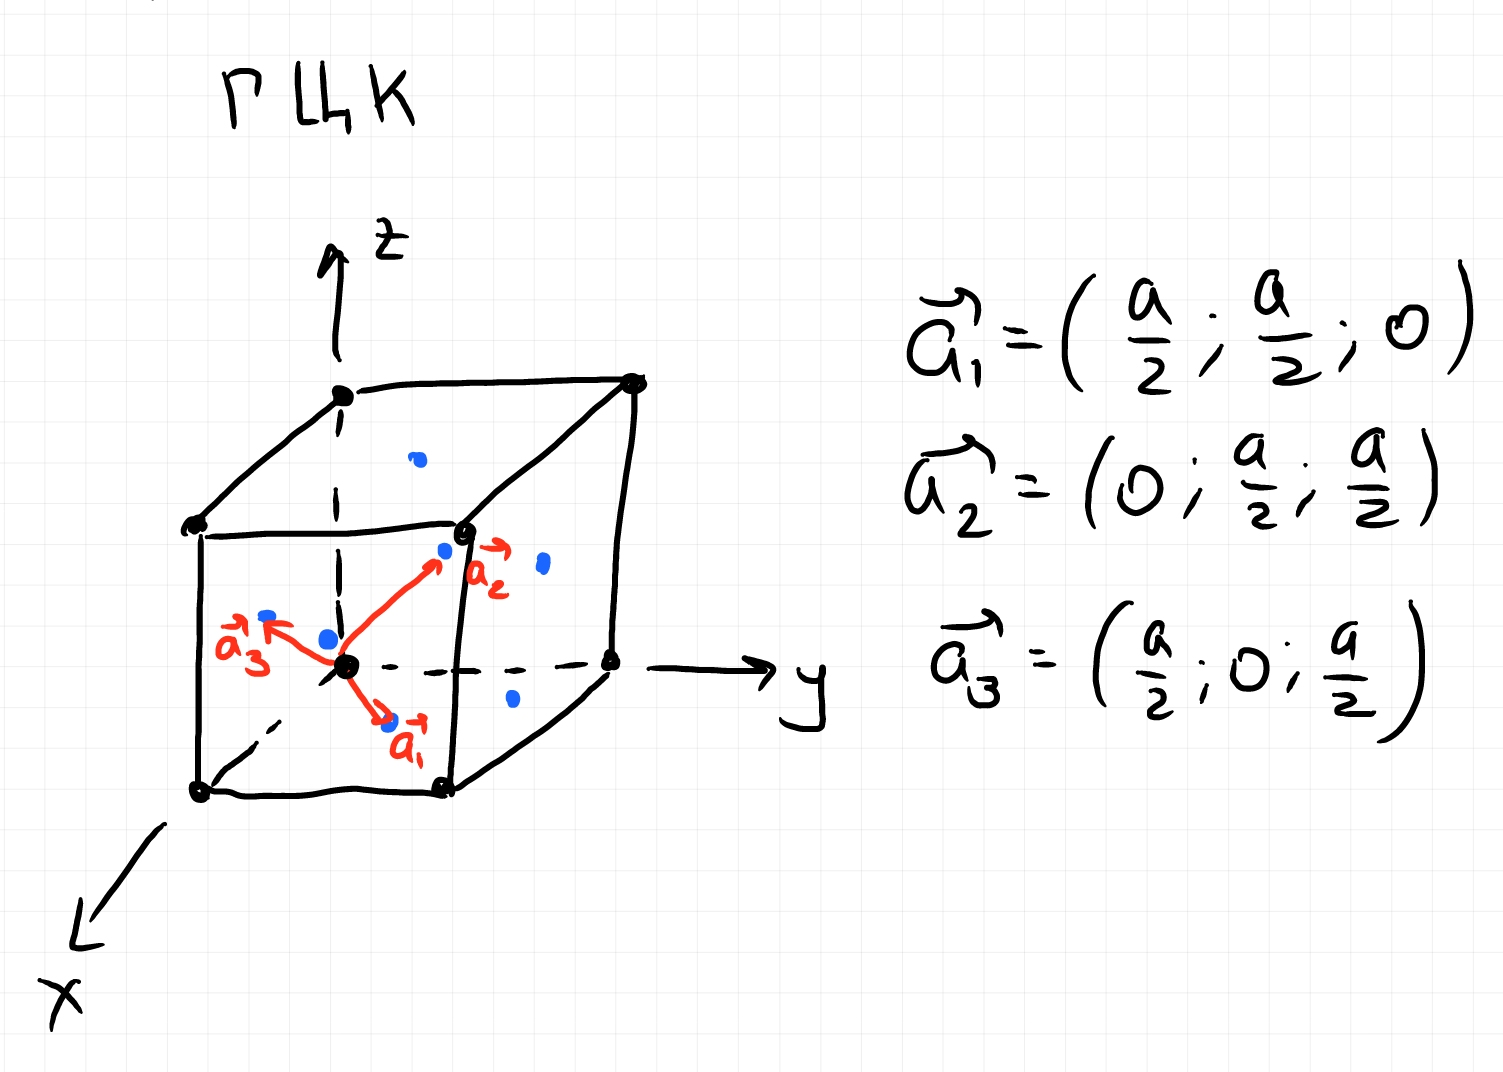
\includegraphics[width=0.8\textwidth]{photo_31.jpg}
\par
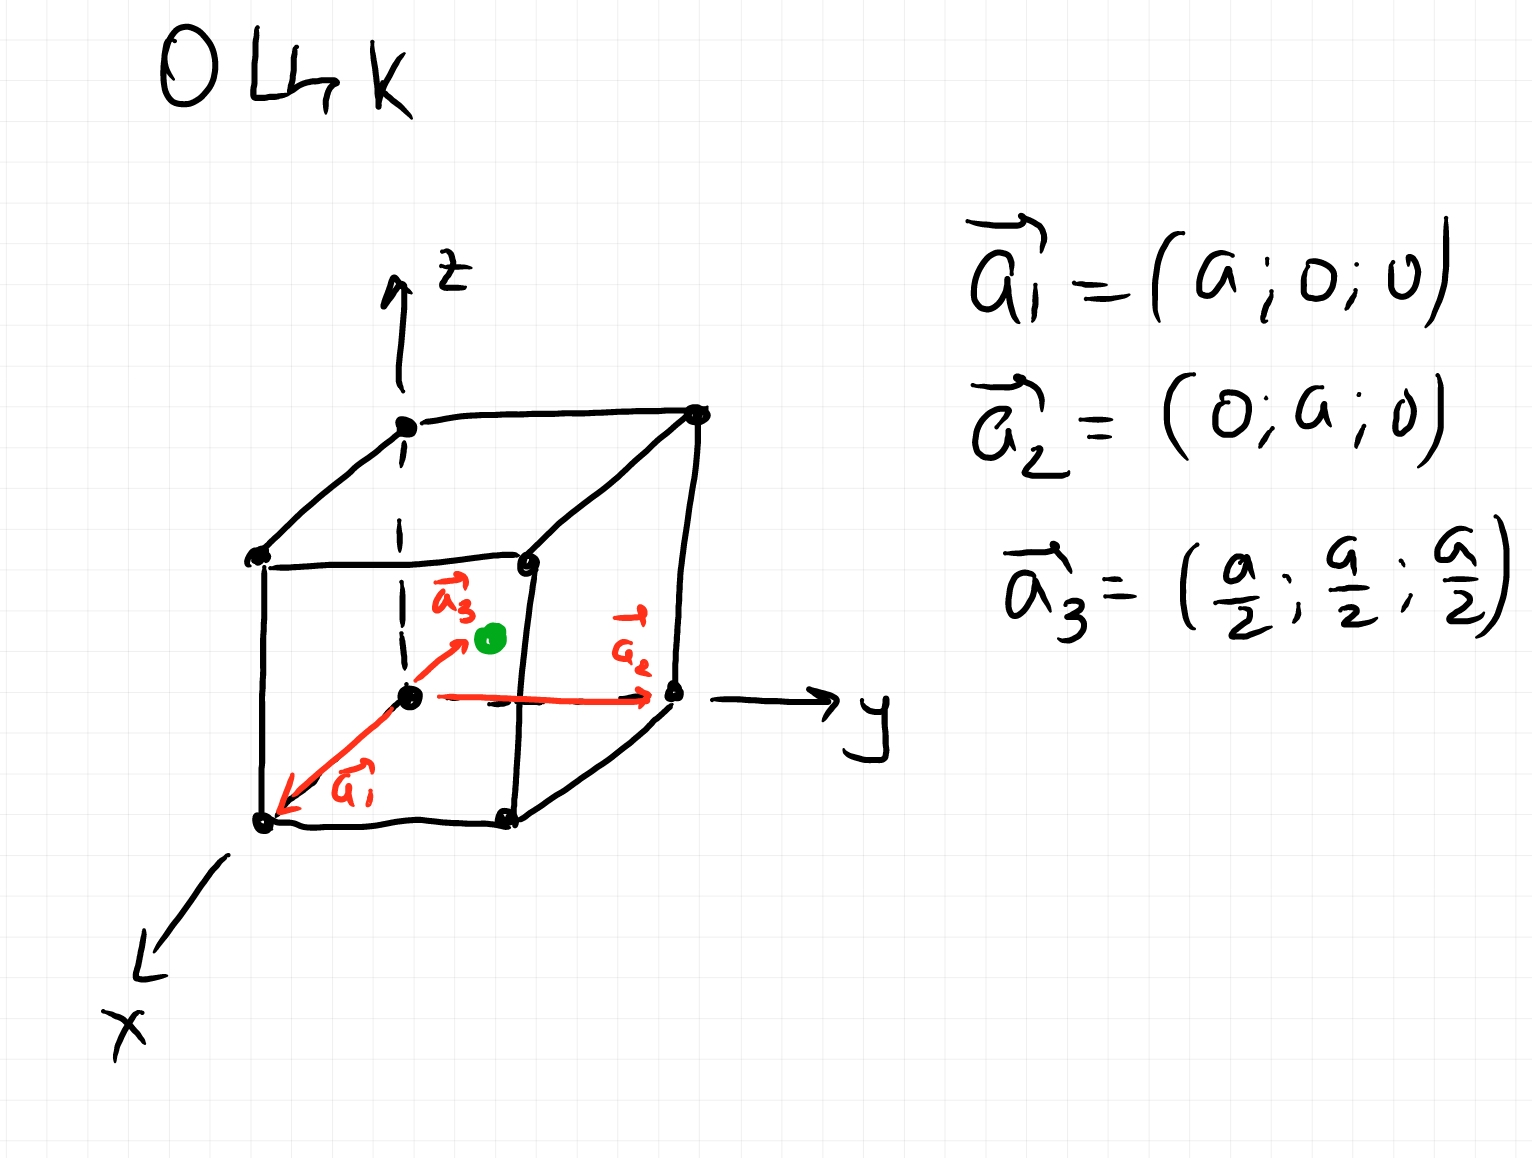
\includegraphics[width=0.8\textwidth]{photo_32.jpg}

\par \textbf{Задача 4}:
\par Условие:
\par
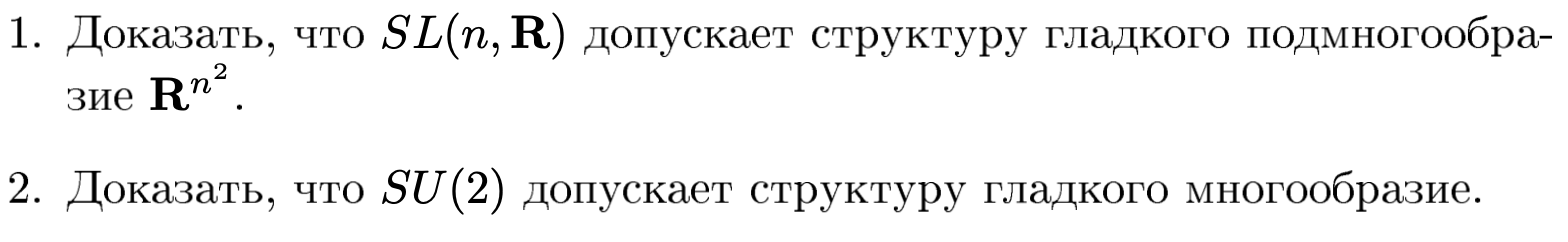
\includegraphics[width=1\textwidth]{photo_4.png}
\par Решение:
\par 1) Кремний, алмаз, поваренная соль - имеют ГЦК решетку с точечной группой $O_h$.
\par Элементы группы:
\[
    E; 8C_3; 6C_2; 6C_4; 3C_2; I; 6S_4; 8S_6; 3\sigma_h; 6\sigma_d
\]
\par Классы сопряженности:
\[
    A_{1g}; A_{2g}; E_g; T_{1g}; T_{2g}; A_{1u}; A_{2u}; E_u; T_{1u}; T_{2u}
\]
\par Представления
\par
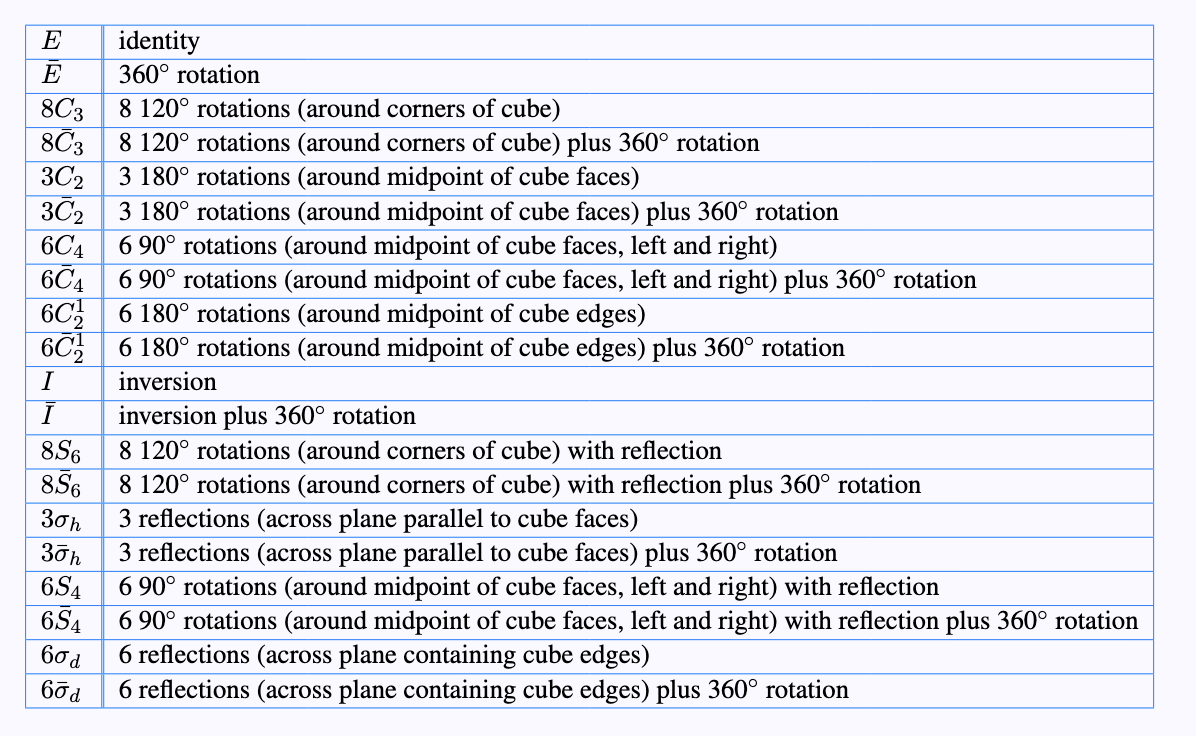
\includegraphics[width=1\textwidth]{Oh.png}
\par
\par 2) Нитрид бора - имеет гексоганальную решетку с точечной группой $D_{6h}$.
\par Элементы группы:
\[
    E; 2C_6; 2C_3; C_2; 3C'_2; 3C''_2; I; 2S_3; 2S_6; \sigma_h; 3\sigma_d; 3\sigma_v
\]
\par Классы сопряженности:
\[
    A_{1g}; A_{2g}; B_{1g}; B_{2g}; E_{1g}; E_{2g}; A_{1u}; A_{2u}; B_{1u}; B_{2u}; E_{1u}; E_{2u}
\]
\par Представления
\par
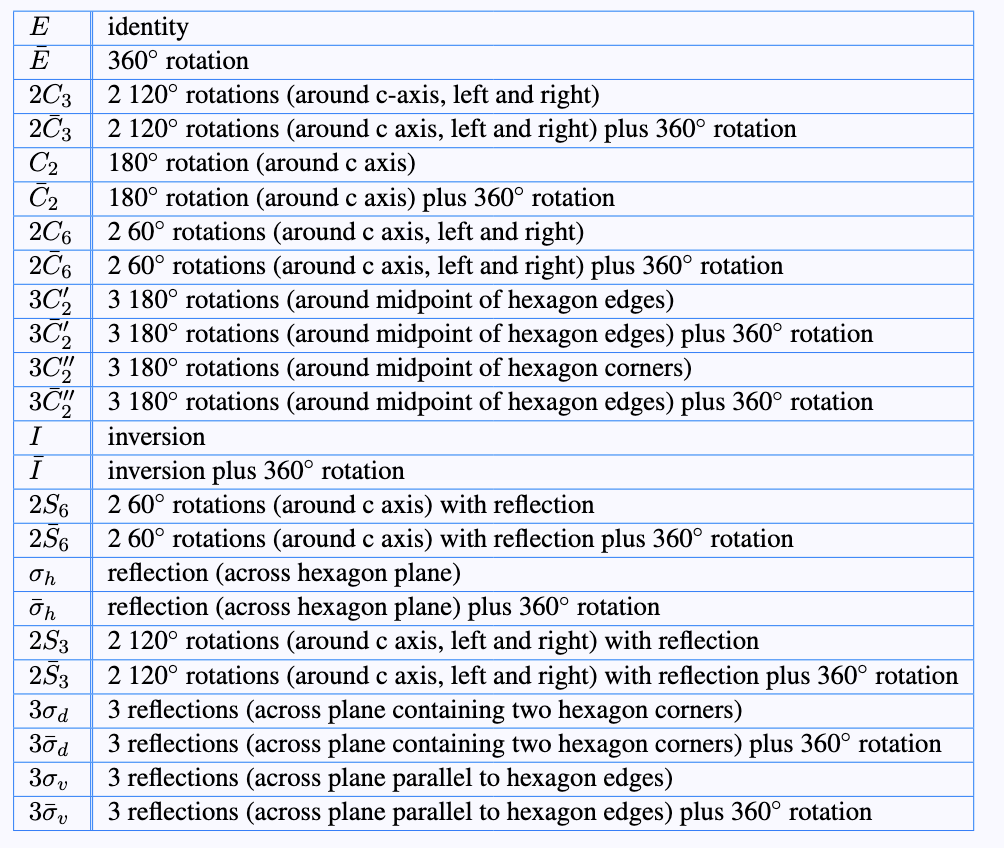
\includegraphics[width=1\textwidth]{D_6h.png}
\par
\par 3) Арсенид галлия - имеет ГЦК решетку с точечной группой $T_{d}$.
\par Элементы группы:
\[
    E; 2C_6; 8C_3; 3C_2; 6S_4; 6\sigma_d
\]
\par Классы сопряженности:
\[
    A_{1}; A_{2}; E; T_{1}; T_{2}
\]
\par Представления
\par
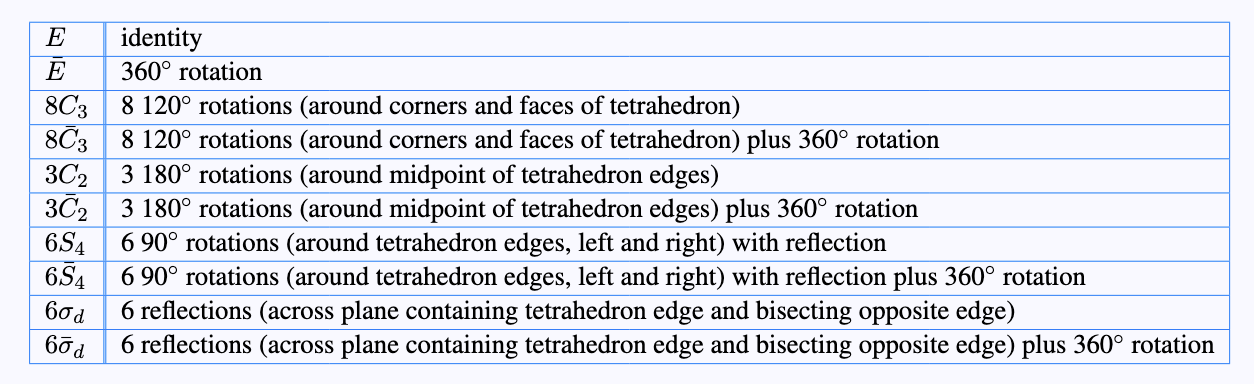
\includegraphics[width=1\textwidth]{Td.png}
\par
\par 4) Нитрид галлия - имеет гексоганальную решетку с точечной группой $C_{6v}$.
\par Элементы группы:
\[
    E; 2C_6; 2C_3; C_2; 3\sigma_d; 3\sigma_v
\]
\par Классы сопряженности:
\[
    A_{1}; A_{2}; B_{1}; B_{2}; E_{1}; E_{2}
\]
\par Представления
\par
\includegraphics[width=1\textwidth]{С_6v.png}
\par
\par 5) Теллур - имеет гексоганальную решетку с точечной группой $D_{3}$.
\par Элементы группы:
\[
    E; 3C_3; 3C'_2
\]
\par Классы сопряженности:
\[
    A_{1}; A_{2}; E
\]
\par Представления
\par
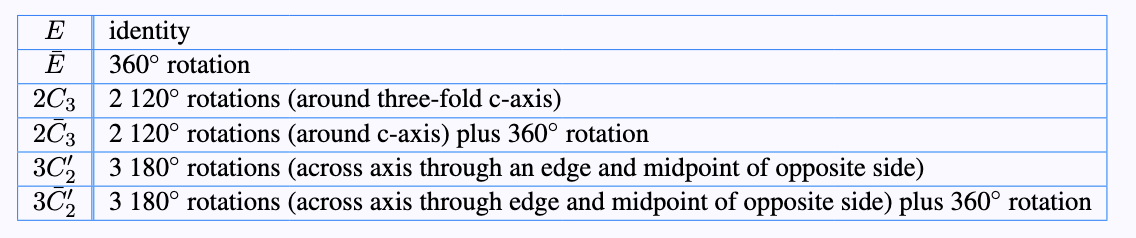
\includegraphics[width=1\textwidth]{D_3.png}
\par

\par
\par \textbf{Задача 5}:
\par Условие:
\par
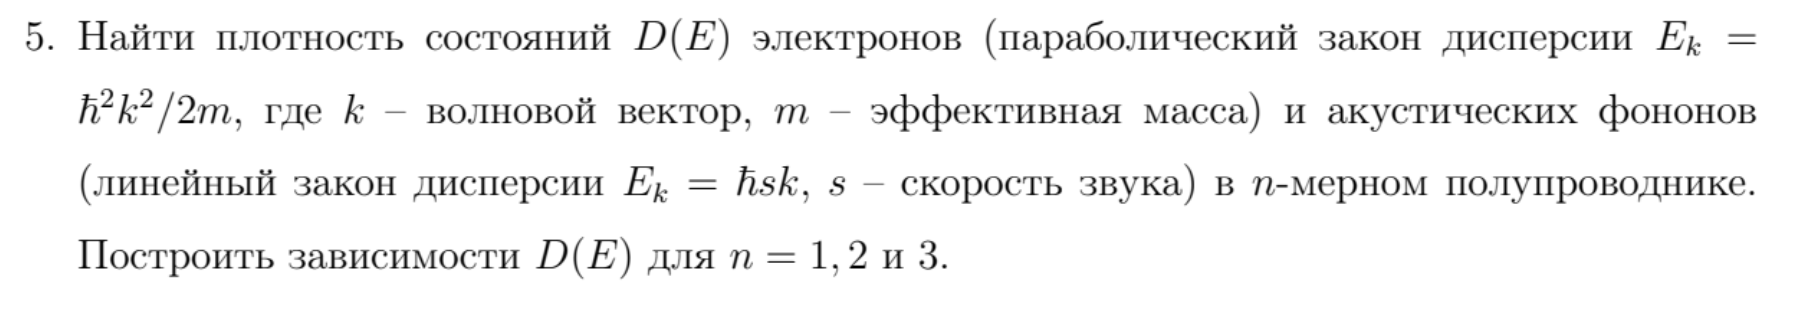
\includegraphics[width=1\textwidth]{photo_5.png}
\par Решение:
\par
\[
    D(E) = g \frac{1}{v} \frac{v}{(2\pi)^n} \int d^{n}k \delta (E-E(k)) =
\]
\[
    = g \frac{1}{(2\pi)^n} S_n \int k^{n-1}dk \delta (k-k(E)) \left| \frac{dk}{dE} \right| =
\]
\par $S_n$ - площадь (n-1) сферы в n-мерном пр-ве; $S_n = \frac{2 \pi^{n/2}}{\Gamma (n/2)}$
\[
    = g \frac{1}{(2\pi)^n} \frac{2\pi^{n/2}}{\Gamma (n/2)} k(E)^{n-1} \left| \frac{dk}{dE} \right|
\]
\par для электрона $E = \frac{\hbar^2 k^2}{2m}$; $k = \left( \frac{2mE}{\hbar^2} \right)^{1/2}$; $\frac{dk}{dE} = \left( \frac{m}{2\hbar^2 E} \right)^{1/2}$
\[
    D(E) = g \frac{1}{2^{n-1} \pi^{n/2} \Gamma (n/2)} \left( \frac{2mE}{\hbar^2} \right)^{\frac{n-1}{2}} \left( \frac{m}{2E\hbar^2} \right)^{\frac{1}{2}}
\]
\[
    n=1: D(E) \sim \frac{1}{\sqrt{E}}
\]
\[
    n=2: D(E) \sim const(E)
\]
\[
    n=3: D(E) \sim \sqrt{E}
\]
\par для фотона $E = \hbar s k$; $k = \frac{E}{s \hbar}$; $\frac{dk}{dE} = \frac{1}{\hbar s}$
\[
    D(E) = g \frac{1}{2^{n-1} \pi^{n/2} \Gamma (n/2)} \left( \frac{E}{s \hbar} \right)^{n-1} \frac{1}{\hbar s}
\]
\[
    n=1: D(E) \sim const(E)
\]
\[
    n=2: D(E) \sim E
\]
\[
    n=3: D(E) \sim E^2
\]
\par

\par \textbf{Задача 6}:
\par Условие:
\par
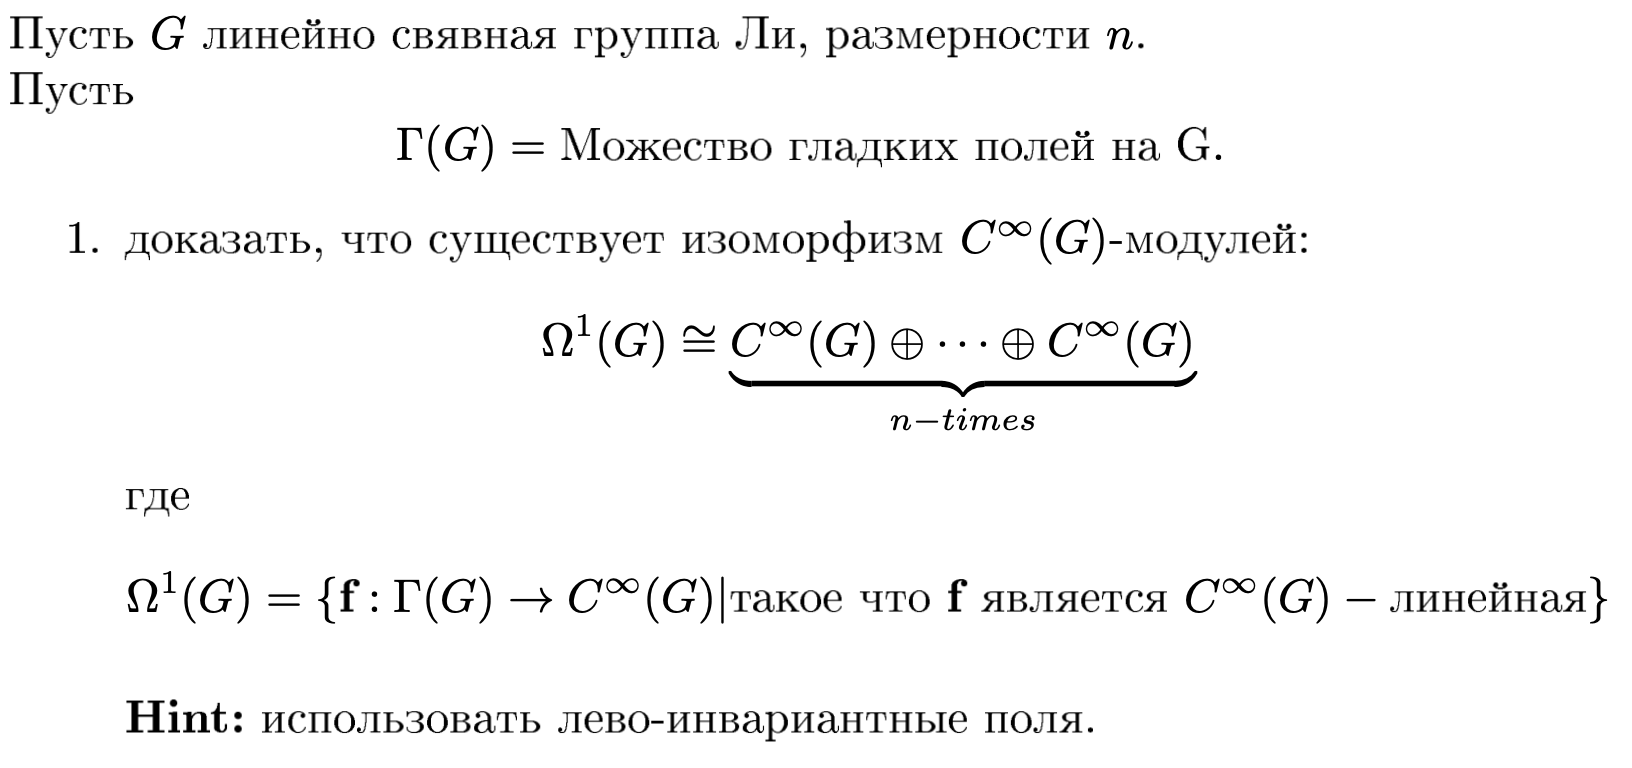
\includegraphics[width=1\textwidth]{photo_6.png}
\par Решение:
\par $E = \sqrt{\left( \frac{E_g}{2} \right)^2 + \left( P k \right)}$; $k = \left( \frac{E^2 - E_g^2/4}{P^2} \right)^{1/2}$; $\frac{dk}{dE} = \frac{E}{P^2}\left( \frac{E^2 - E_g^2/4}{P^2} \right)^{-1/2}$; $n=3$
\[
    D(E) = g \frac{1}{4 \pi^{3/2} \Gamma (3/2)} \frac{E}{P^2}\left( \frac{E^2 - E_g^2/4}{P^2} \right)^{1/2}
\]
\[
    \Gamma(3/2) = \frac{sqrt{\pi}}{2} ; \,\, g = 2s+1 = 2
\]
\[
    D(E) = \frac{1}{\pi^2} \frac{E}{P^2}\left( \frac{E^2 - E_g^2/4}{P^2} \right)^{1/2}
\]
\par

\par \textbf{Задача 7}:
\par Условие:
\par
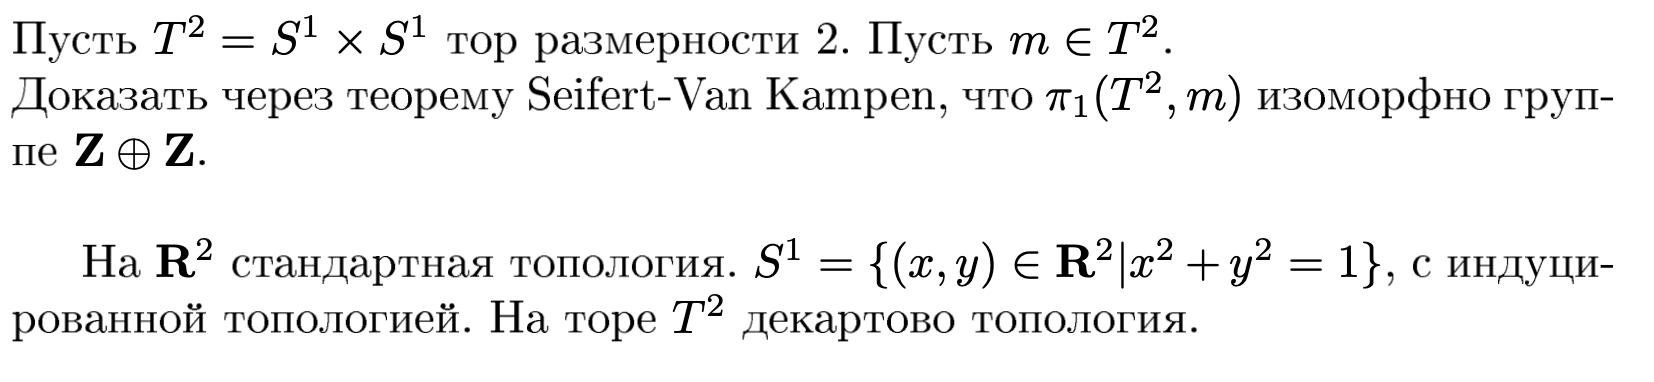
\includegraphics[width=1\textwidth]{photo_7.png}
\par Решение:
\par :(
\par

\par \textbf{Задача 8}:
\par Условие:
\par
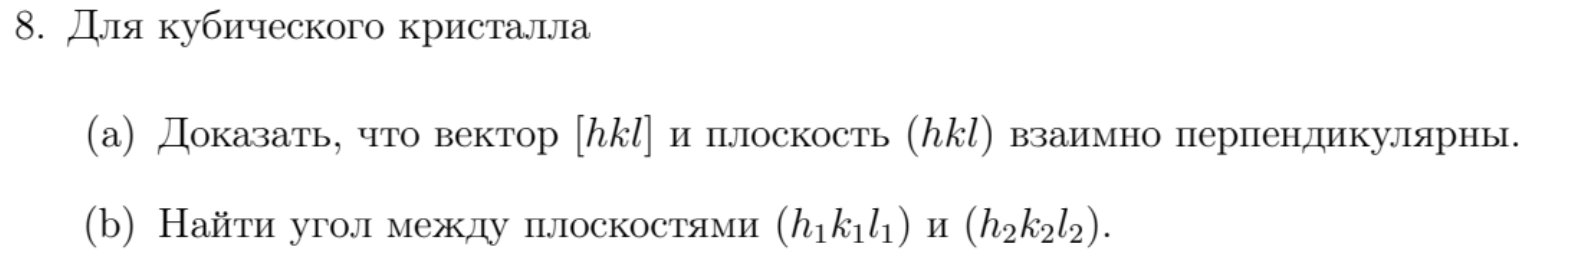
\includegraphics[width=1\textwidth]{photo_8.png}
\par Решение:
\par 1) Кубический кристалл:
\[
    \vec{a_1} \perp \vec{a_2} \perp \vec{a_3}
\]
\[
    |\vec{a_1}| = |\vec{a_2}| = |\vec{a_3}|
\]
\[
    \vec{g} = \sum_{i} g_i \vec{a_i} \,; \,\, g_1; g_2; g_3 = h; k; l
\]
\par Из курса Никиты Сергеевича знаем, что все вектора в плоскости можно представить ввиде суммы векторов:
\[
    \vec{c_1} = \frac{\vec{a_1}}{h} - \frac{\vec{a_2}}{k} \, ; \,\, \vec{c_2} = \frac{\vec{a_1}}{h} - \frac{\vec{a_3}}{l} \, ; \,\, \vec{c_3} = \frac{\vec{a_2}}{k} - \frac{\vec{a_3}}{l}
\]
\[
    \vec{g} \cdot \vec{c_1} = \frac{g_1 \vec{a_1}\cdot\vec{a_1}}{h} -  \frac{g_2 \vec{a_2}\cdot\vec{a_2}}{k} = |\vec{a_1}|^2 - |\vec{a_2}|^2 = 0
\]
\par ан-но для $\vec{c_1}; \vec{c_2}$
\par QED
\par 2) из прошлого пунка теперь знаем что угол между плоскостями $(h_1 k_1 l_1)$ и $(h_2 k_2 l_2)$ равен углу между векторами $[h_1 k_1 l_1]$ и $[h_2 k_2 l_2]$
\[
    \cos \alpha = \frac{|h_1 h_2 + k_1 k_2 + l_1 l_2|}{\sqrt{h_1^2 + k_1^2 + l_1^2} \sqrt{h_2^2 + k_2^2 + l_2^2}}
\]
\par
\par \textbf{Задача 9}:
\par Условие:
\par
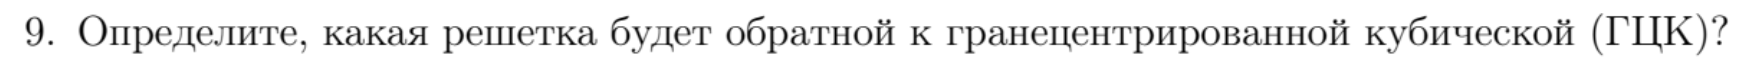
\includegraphics[width=1\textwidth]{photo_9.png}
\par Решение:
\par
\[
    \vec{b_1} = \frac{2\pi}{v_0} \left[ \vec{a_2} \times \vec{a_3} \right]
\]
\[
    \vec{b_2} = \frac{2\pi}{v_0} \left[ \vec{a_3} \times \vec{a_1} \right]
\]
\[
    \vec{b_3} = \frac{2\pi}{v_0} \left[ \vec{a_1} \times \vec{a_2} \right]
\]
\[
    v_0 = (\vec{a_1} \cdot \left[ \vec{a_2} \times \vec{a_3} \right])
\]
\[
    \text{ГЦК} \Rightarrow \vec{a_1} = \left( a/2; 0; a/2 \right)
\]
\[
    \vec{a_2} = \left( a/2; a/2; 0 \right)
\]
\[
    \vec{a_3} = \left( 0; a/2; a/2 \right)
\]
\[
    \Rightarrow v_0 = \begin{vmatrix}
a/2 & 0 & a/2\\
0 & a/2 & a/2\\
0 & a/2 & a/2
\end{vmatrix} = \frac{a^3}{4}
\]
\[
    \Rightarrow \vec{b_1} = \frac{8\pi}{a^3}  \left( a^2/4; -a^2/4; a^2/4 \right) = \frac{2\pi}{a} \left( 1; -1; 1 \right)
\]
\[
    \vec{b_2} = \frac{8\pi}{a^3}  \left( a^2/4; a^2/4; -a^2/4 \right) = \frac{2\pi}{a} \left( 1; 1; -1 \right)
\]
\[
    \vec{b_3} = \frac{8\pi}{a^3}  \left( -a^2/4; a^2/4; a^2/4 \right) = \frac{2\pi}{a} \left( -1; 1; 1 \right)
\]
\par ОЦК со стороной $b = \frac{4\pi}{a}$

\par
\end{large}
\end{document}
